\section{Enkätresultat och kontinuerliga demonstrationer}

Nedan presenteras resultatet av enkätundersökningen som beskrivs under \ref{sec:method-poll}, både i figur \ref{fig:poll_results} och tabell \ref{tab:poll_results_table}. Detta resultat tillsammans med resultatet från de kontinuerliga demonstrationerna diskuteras senare under \ref{sec:discussion-results}. Resultatet från demonstrationerna för kunden är tyvärr inte kvantitativt på samma sätt som enkätsundersökningen. Feedbacken gruppen fick från kunden användes istället direkt genom att fokusera på de funktioner produkten behövde för att uppfylla kraven. Demonstationerna gav en mer öppen dialog kring implementation och design av produkten och tillät gruppen att direkt implementera kundens önskemål i produkten.

\begin{figure}
    \centering
    \begin{subfigure}[]{0.5\textwidth}
        \centering
        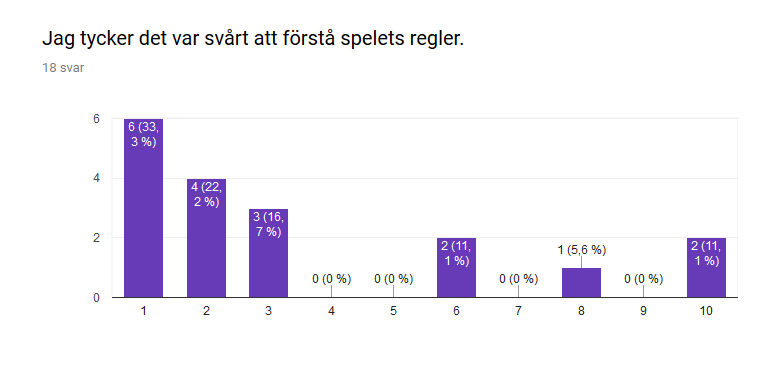
\includegraphics[width=7cm]{poll_results_2}
        \caption{}
    \end{subfigure}%
    ~
    \begin{subfigure}[]{0.5\textwidth}
        \centering
        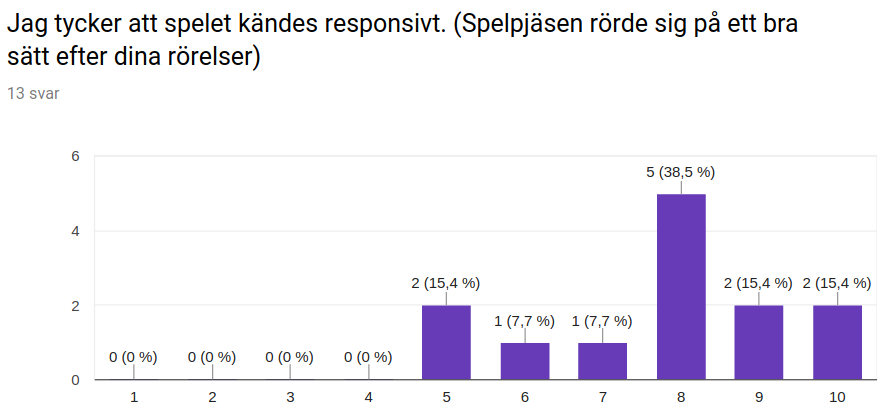
\includegraphics[width=7cm]{poll_results_3}
        \caption{}
    \end{subfigure}

    \begin{subfigure}[]{0.5\textwidth}
        \centering
        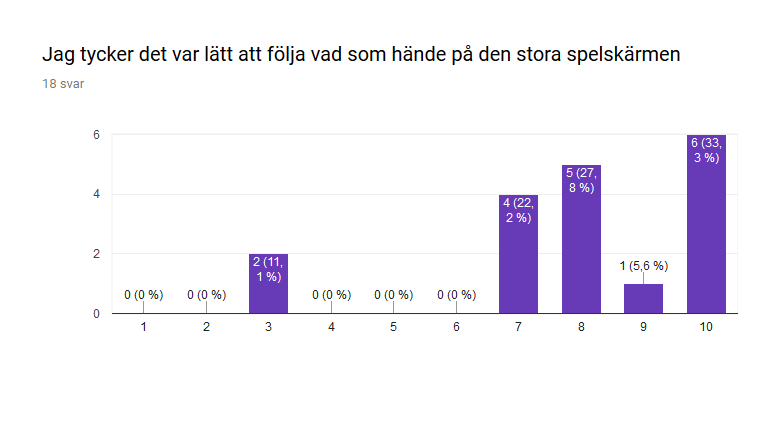
\includegraphics[width=7cm]{poll_results_4}
        \caption{}
    \end{subfigure}%
    ~
    \begin{subfigure}[]{0.5\textwidth}
        \centering
        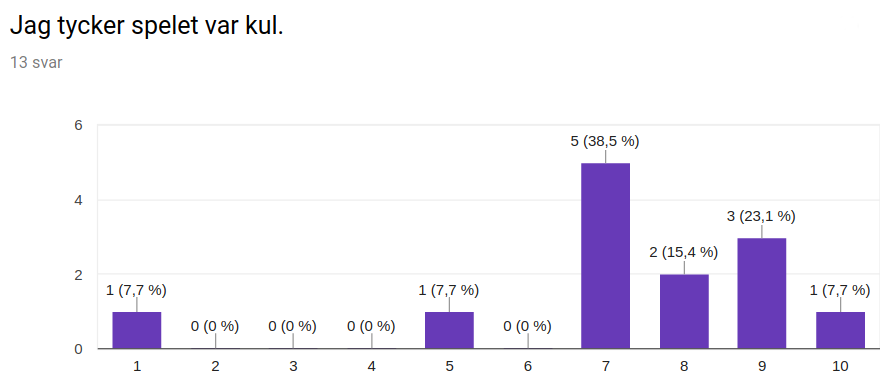
\includegraphics[width=7cm]{poll_results_5}
        \caption{}
    \end{subfigure}

    \begin{subfigure}[]{0.5\textwidth}
        \centering
        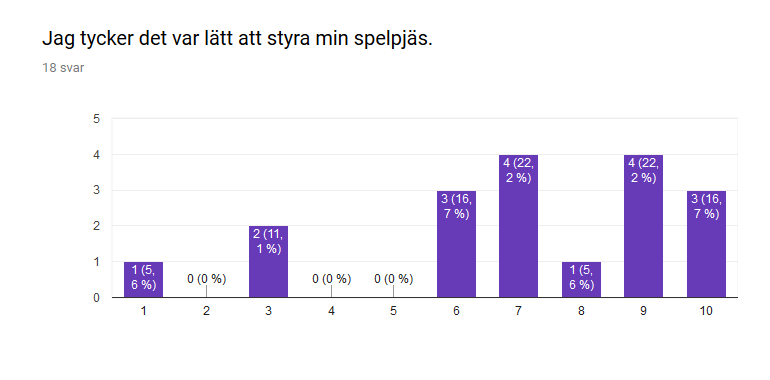
\includegraphics[width=7cm]{poll_results_6}
        \caption{}
    \end{subfigure}%
    \caption{Resultat från enkäten testpersonerna var tillfrågade att fylla i}
    \label{fig:poll_results}
\end{figure}

\begin{table}
    \centering
    \begin{tabular}{| l | l | l | l | l | l |}
        \cline{2-6}
        \multicolumn{1}{c|}{} & (a) & (b) & (c) & (d) & (e) \\ \hline
        Medelvärde & 4.2 & 7.8 & 7.6 & 7.2 & 6.5  \\ \hline
        Median & 3 & 8 & 8 & 7 & 7  \\ \hline
        Standardavvikelse & 3.4 & 1.6 & 2.4 & 2.3 & 2.8  \\ \hline
    \end{tabular}
    \caption{Medelvärden, median och standardavvikelse för resultaten av enkäten}
    \label{tab:poll_results_table}
\end{table}
